%\chapter{External resources}\label{External resources}
\chapter{Resources for Pre-Experiment: Study 1 (\sect{sec:Exp1})}
\label{app:exp1}
The following documents were used in the first user study. As all experiments were conducted in French, all documents are in French:
\begin{itemize}
	\item{Experimental protocol}
	\item{Post-study questionnaire}
	\item{Action schema used}
\end{itemize}
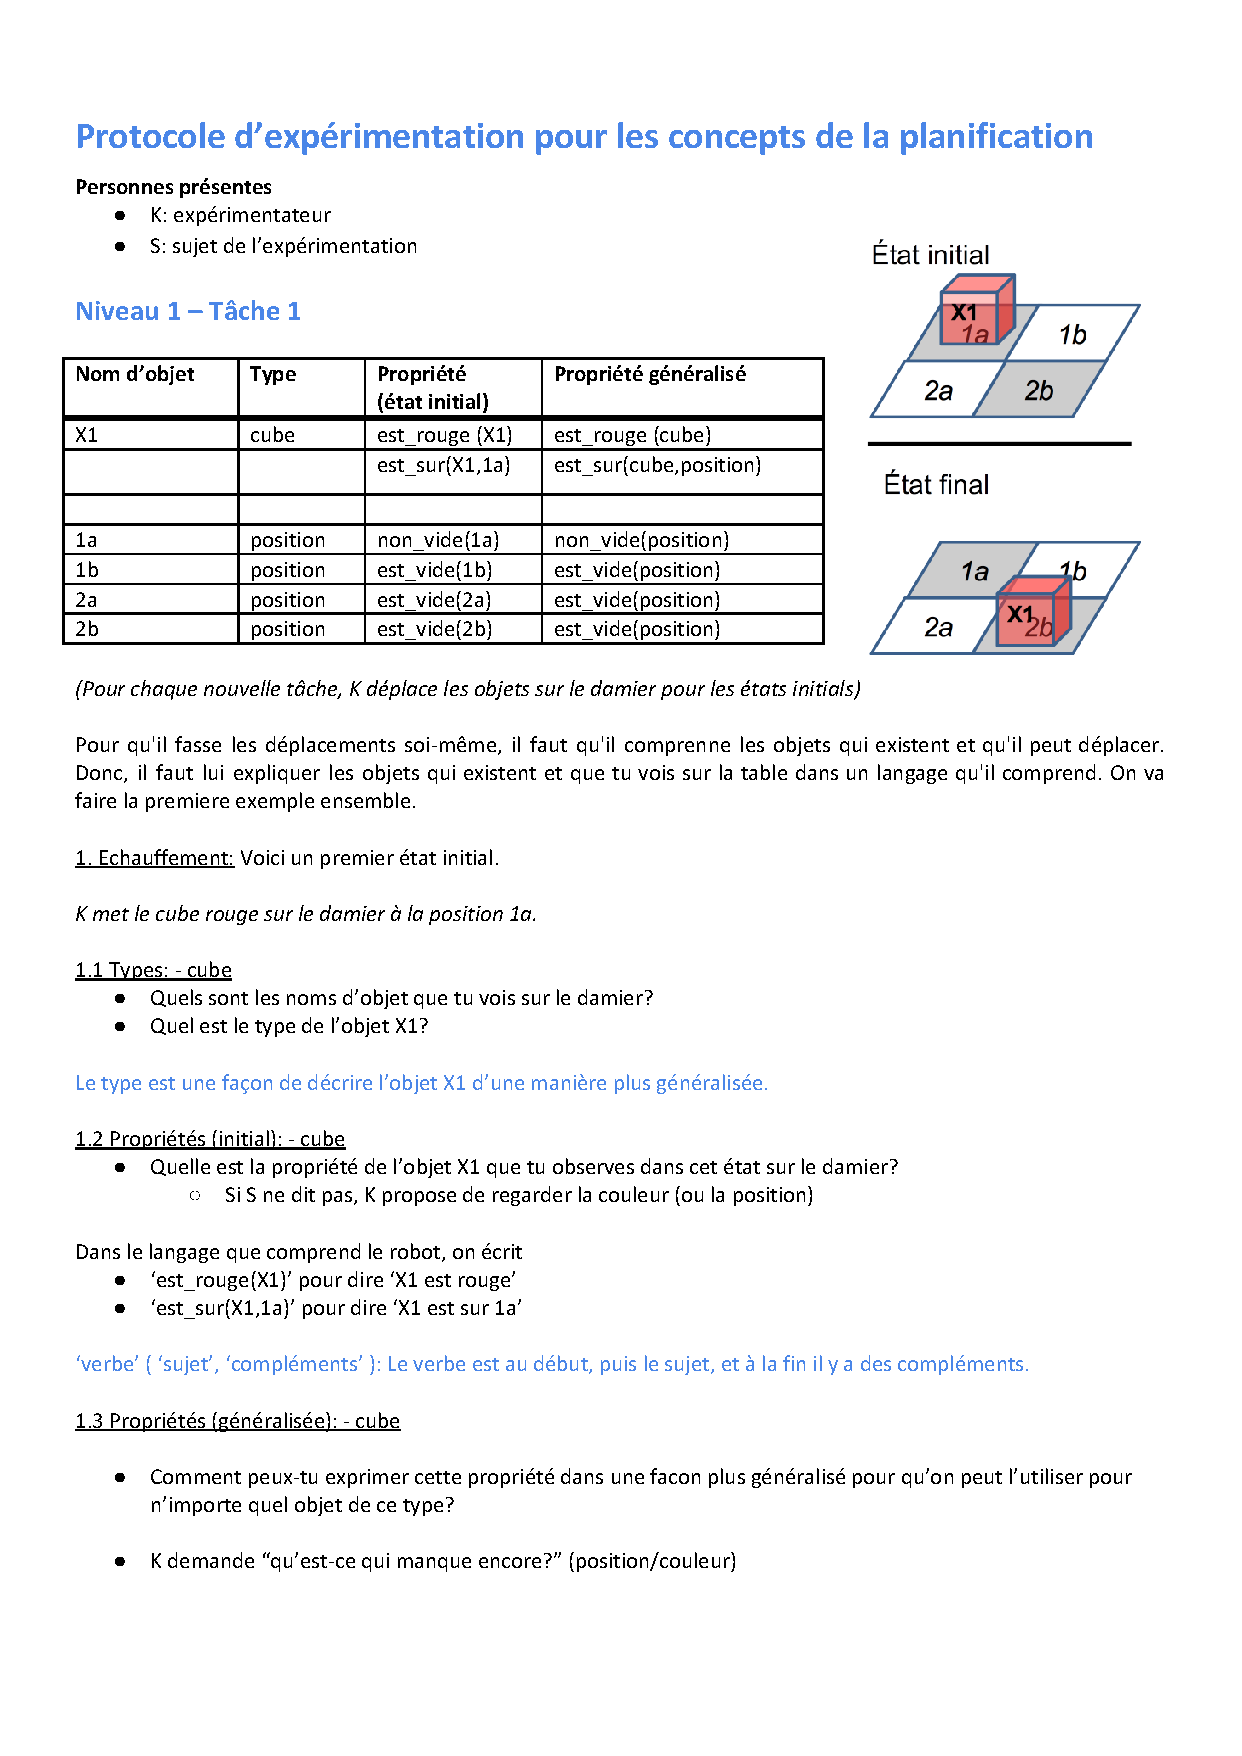
\includepdf[pages=1-6]{7-appendix/exp1-protocole.pdf}
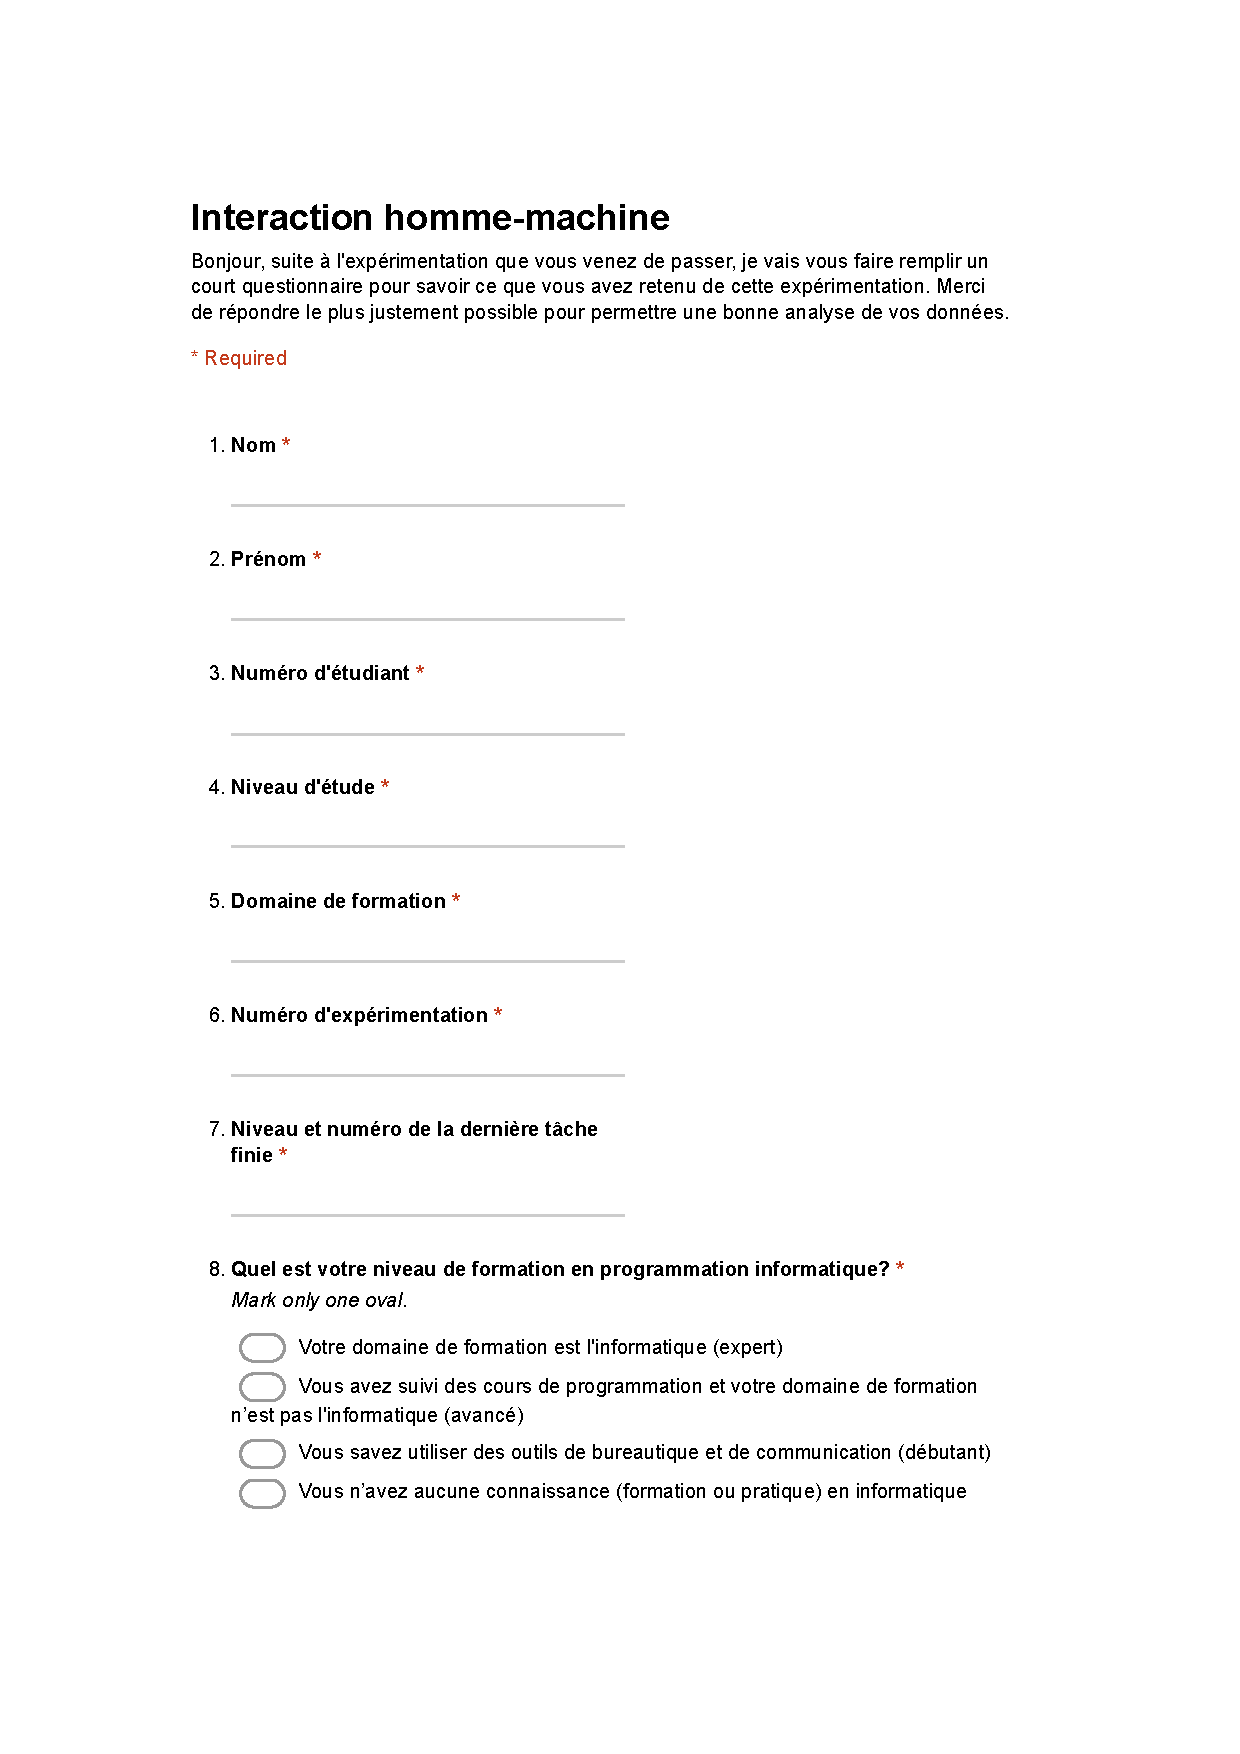
\includepdf[pages=1-7]{7-appendix/exp1-questionnaire.pdf}
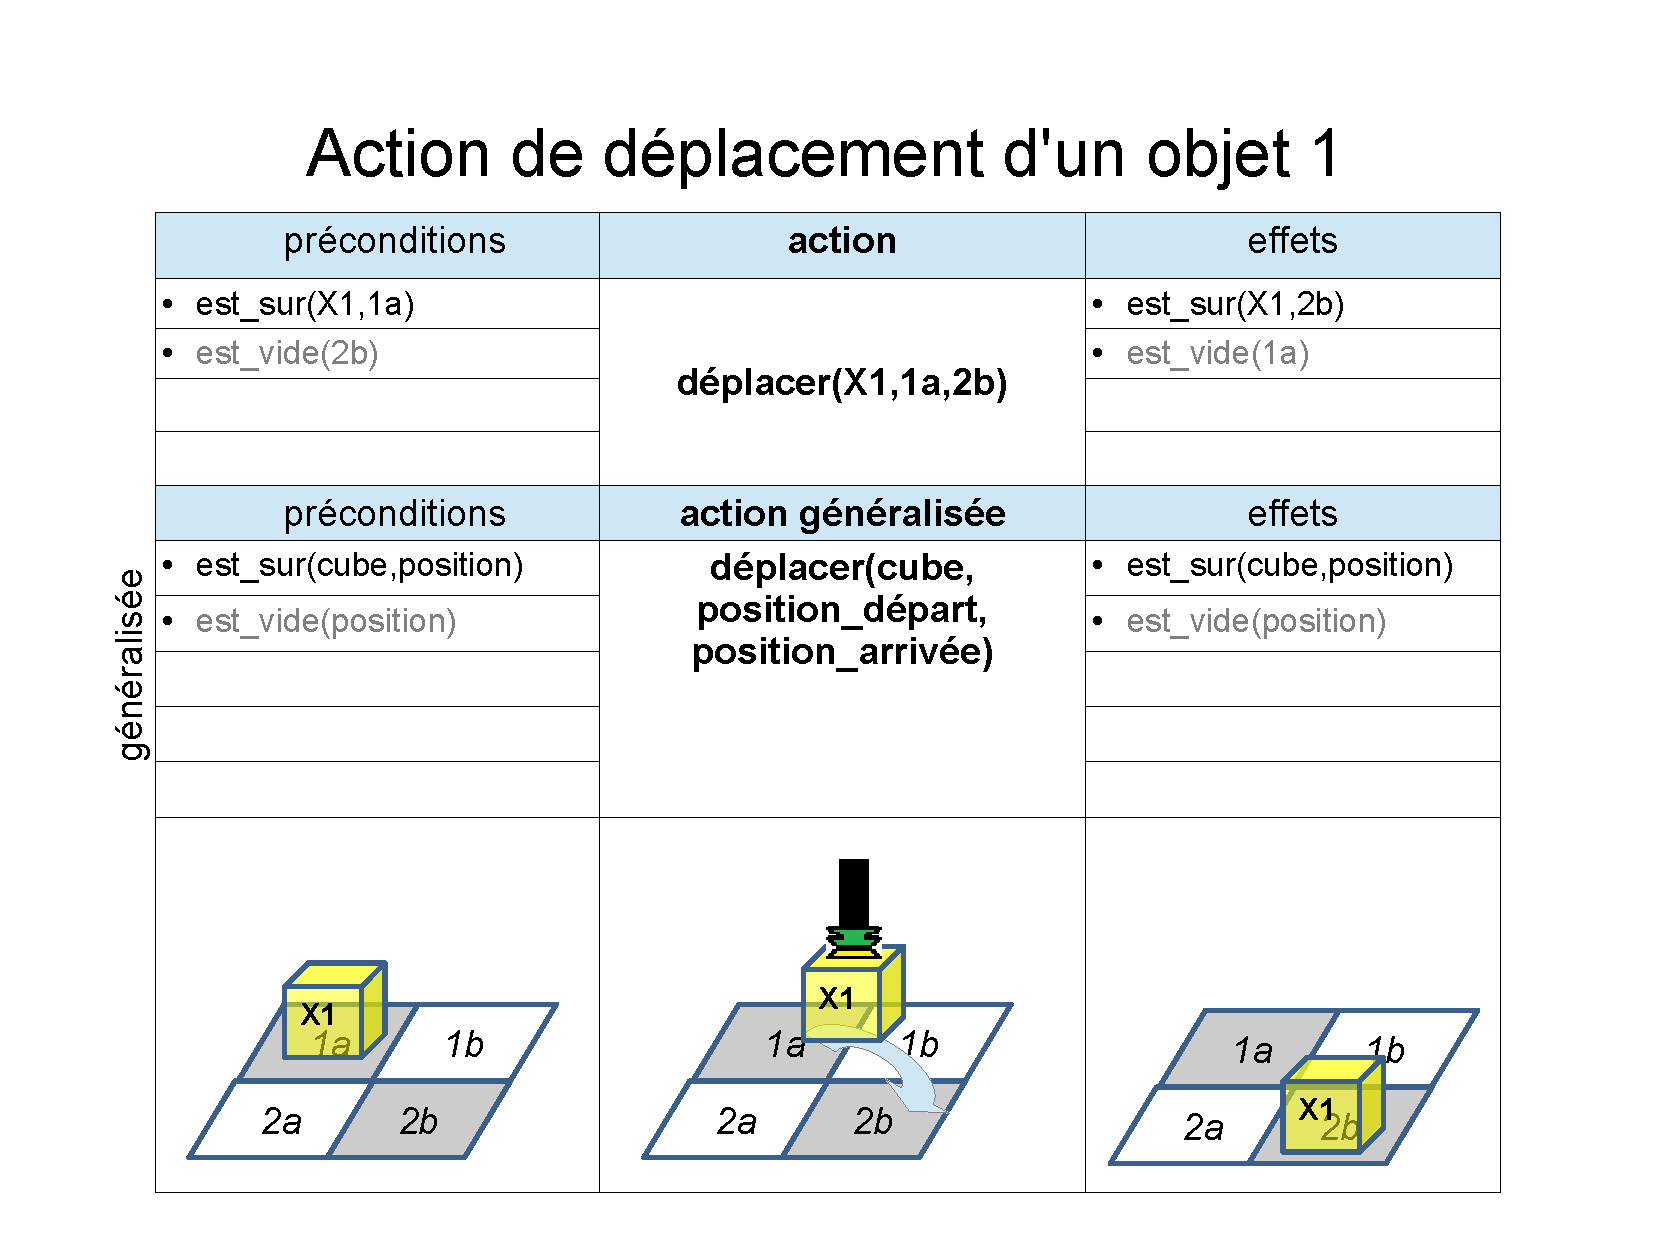
\includepdf[pages=1-4]{7-appendix/exp1-additionalmaterial.pdf}

%\includepdf[pages=1-5]{notes.pdf}

\chapter{Resources for Pre-Experiment: Study 2 (\sect{sec:Exp2}) }
\label{app:exp2}
The following documents were used in the second user study. As all experiments were conducted in French, all documents are in French:
\begin{itemize}
	\item{Experimental protocol}
	\item{Post-study questionnaire}
	\item{Action schema used}
\end{itemize}
A summary of the resources used for this section can be found online:
\begin{itemize}
	\item A demonstration of the Robot Programming process of our proposed framework: \url{https://youtu.be/DTm2YjiSNQM}
	\item The source code for the system implemented using the Wizard-of-Oz technique can be found online: \url{https://github.com/ysl208/Baxter_PbD/}
\end{itemize}

%\section{Experimental protocol (In French)}
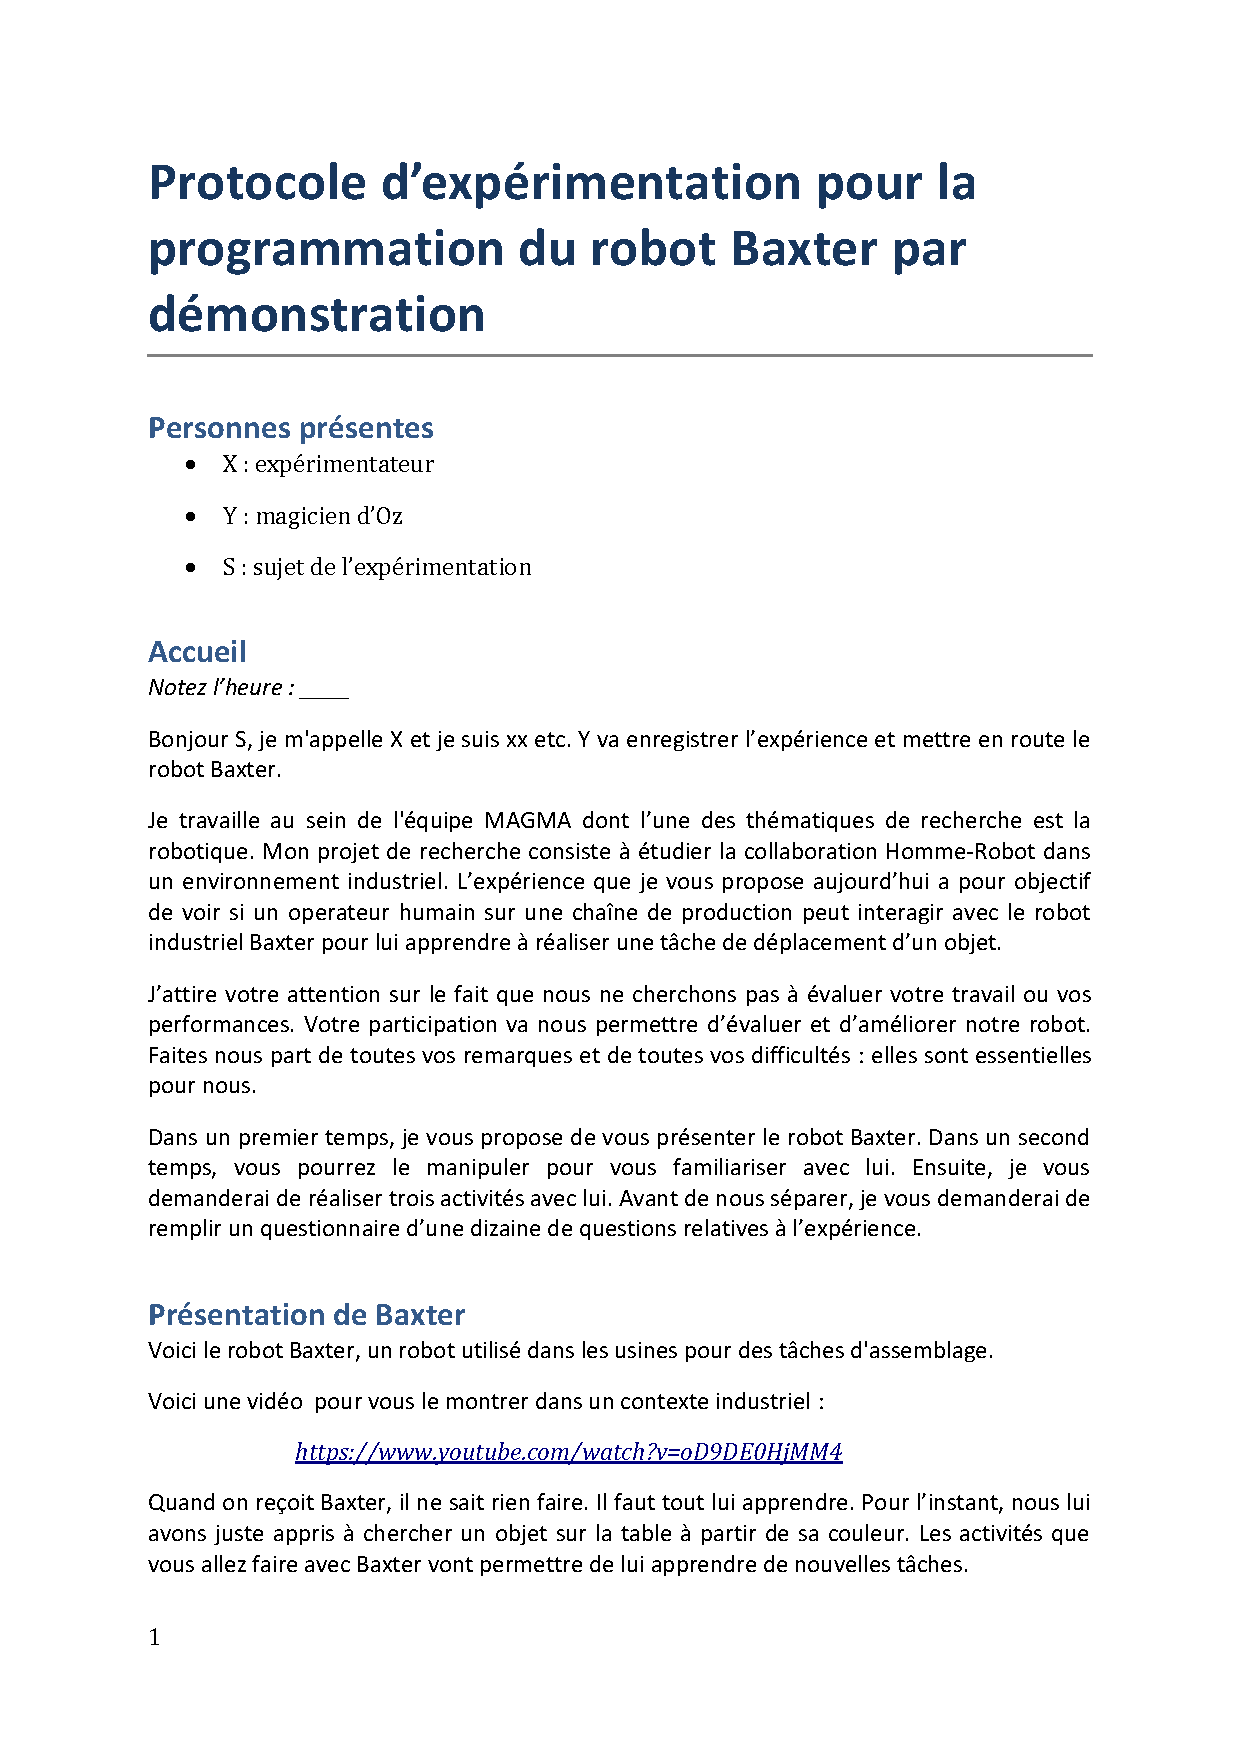
\includepdf[pages=1-7]{7-appendix/exp2-protocole.pdf}
%\section{Questionnaire (In French)}
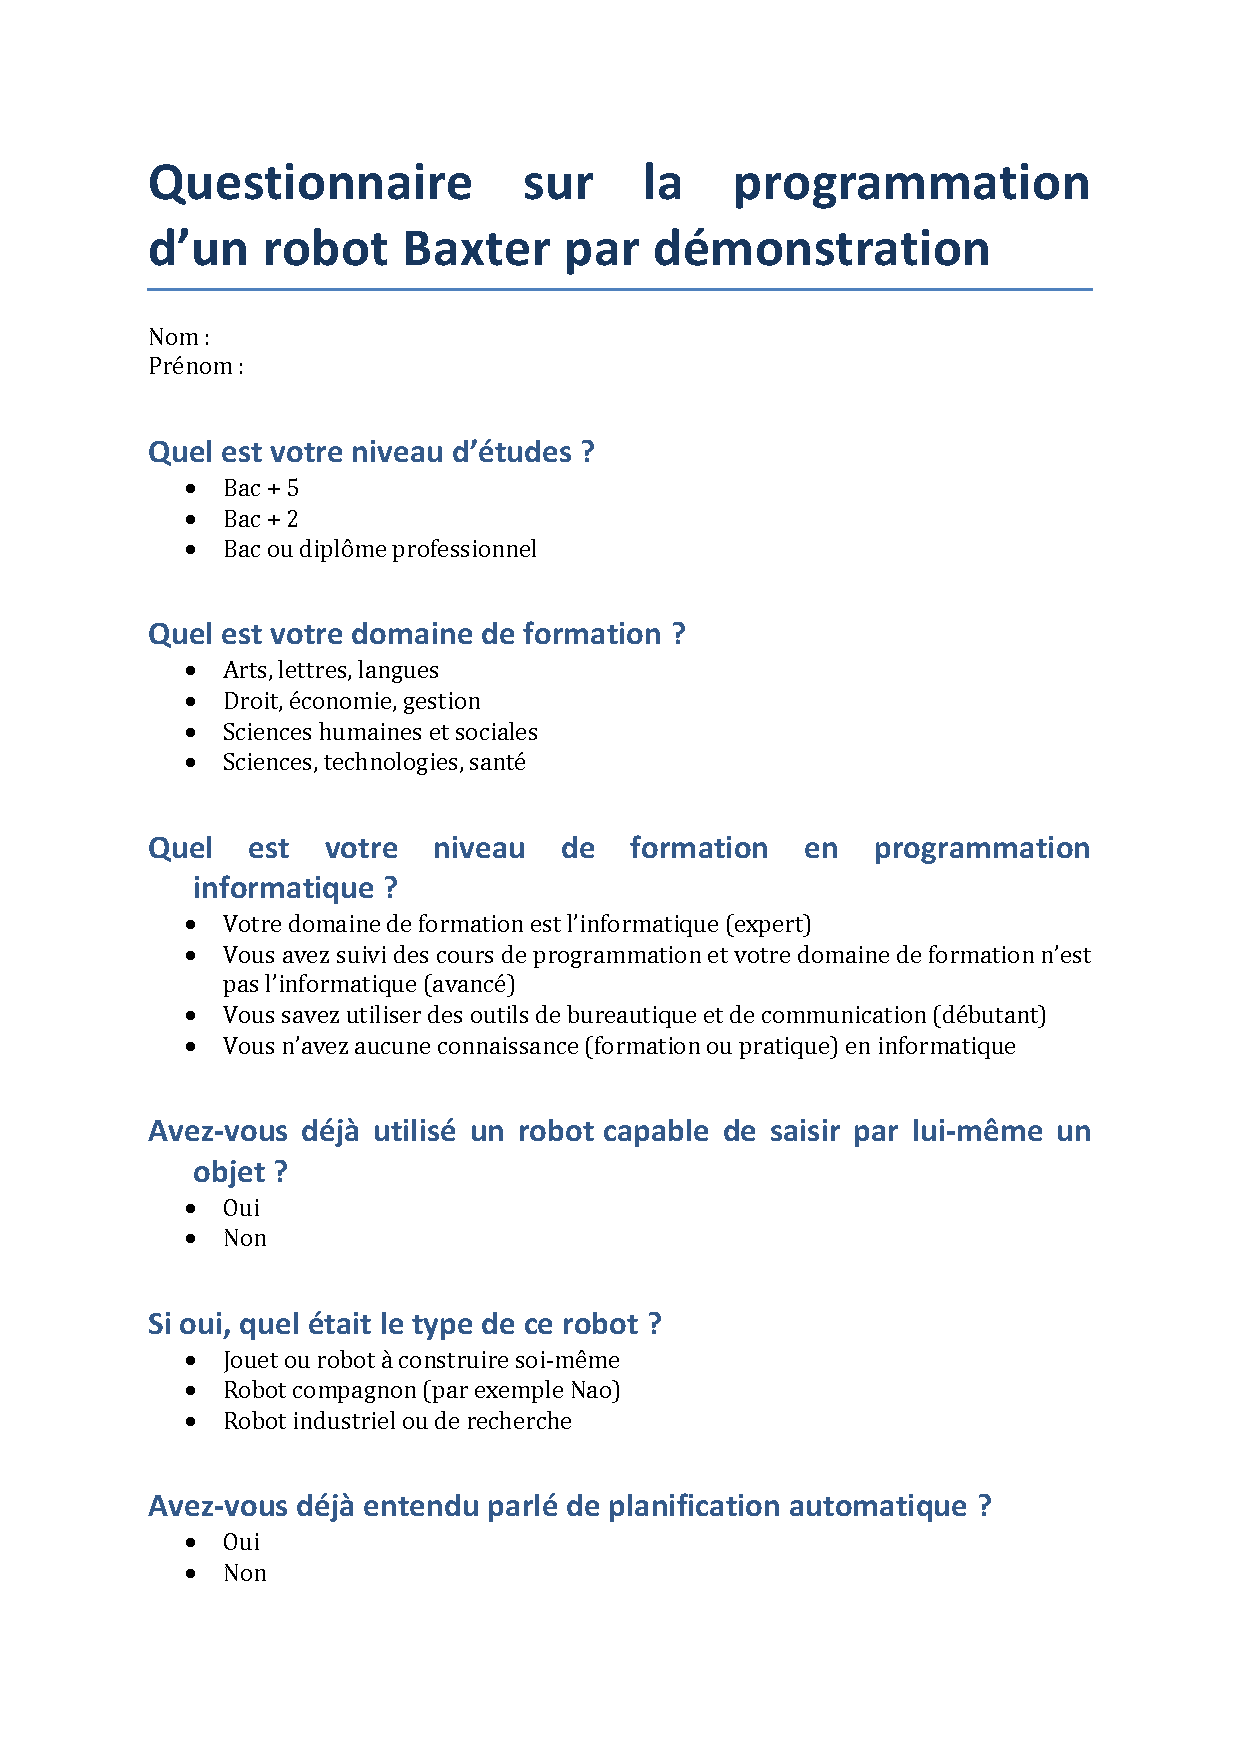
\includepdf[pages=1-3]{7-appendix/exp2-questionnaire.pdf}
%%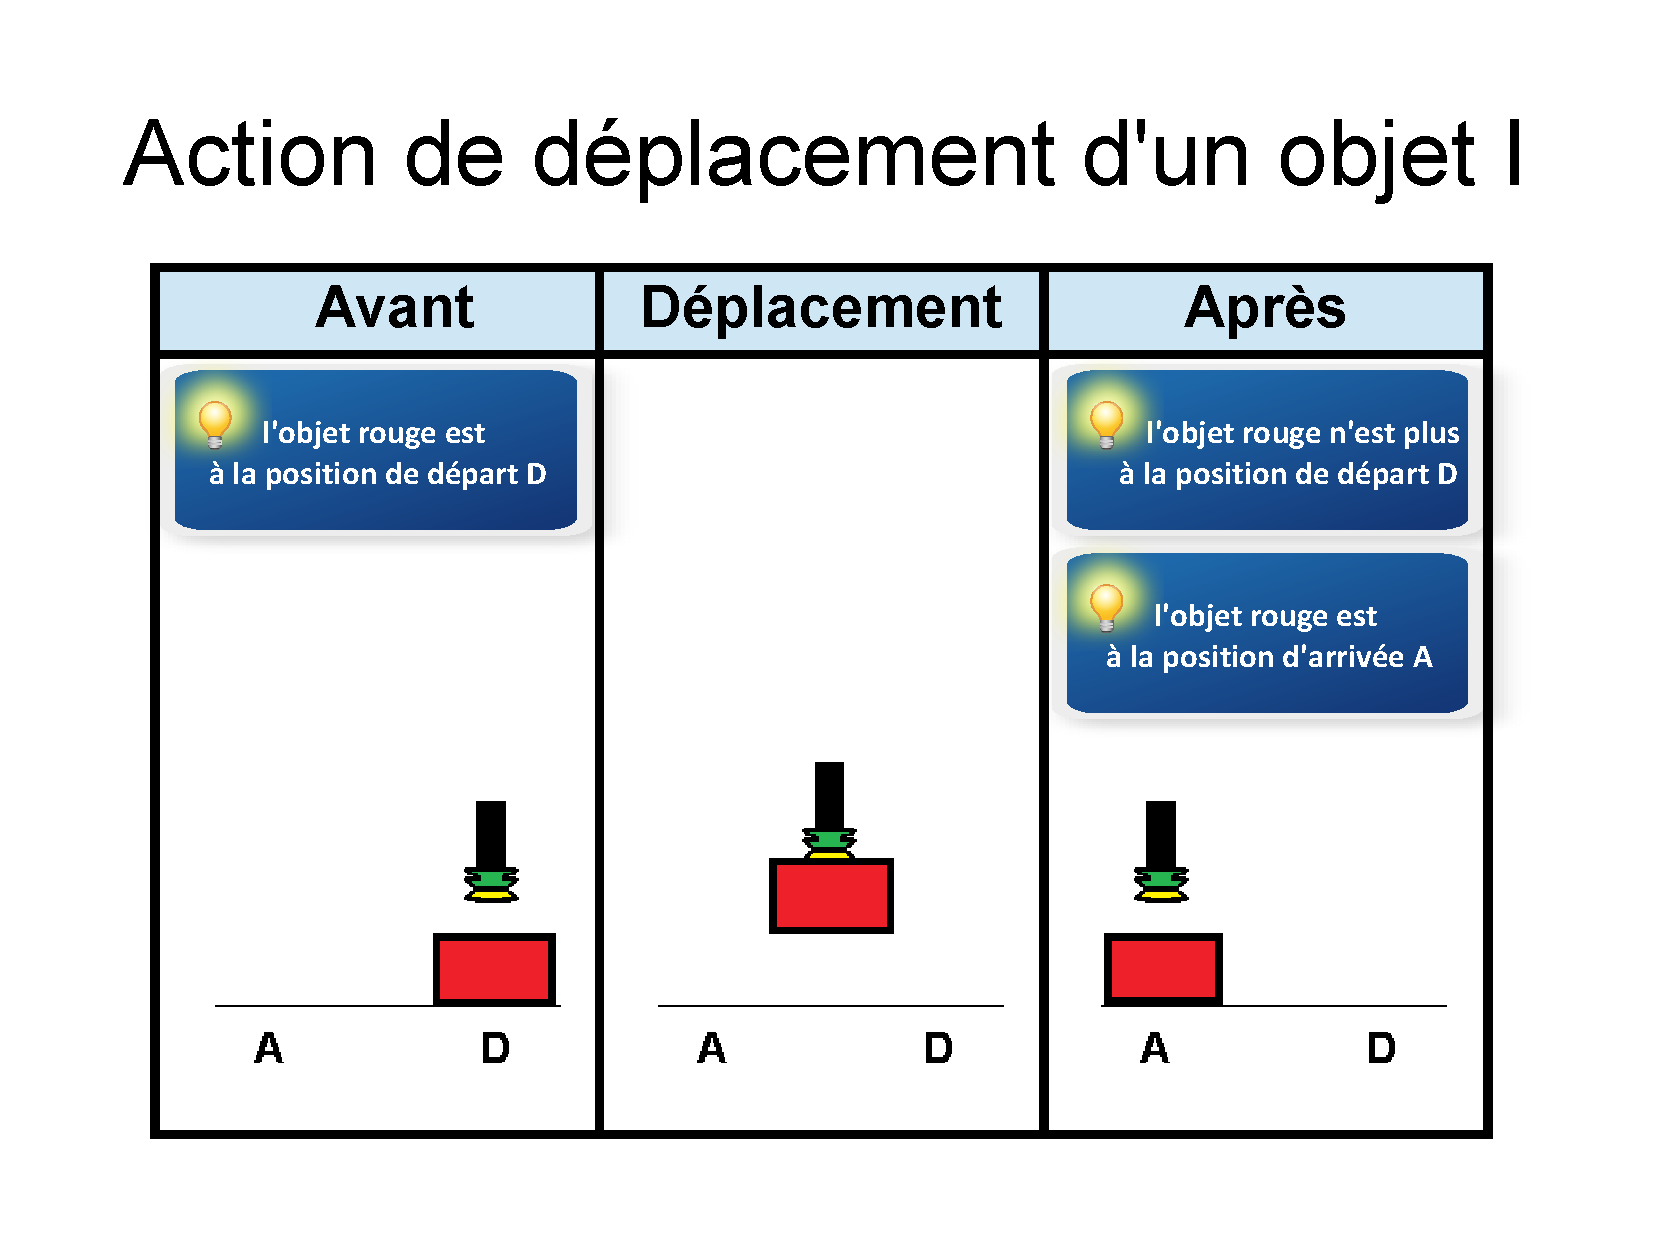
\includepdf[pages=1-3]{7-appendix/exp2-additionalmaterial.pdf}
  \begin{figure}[h]
    \centering
    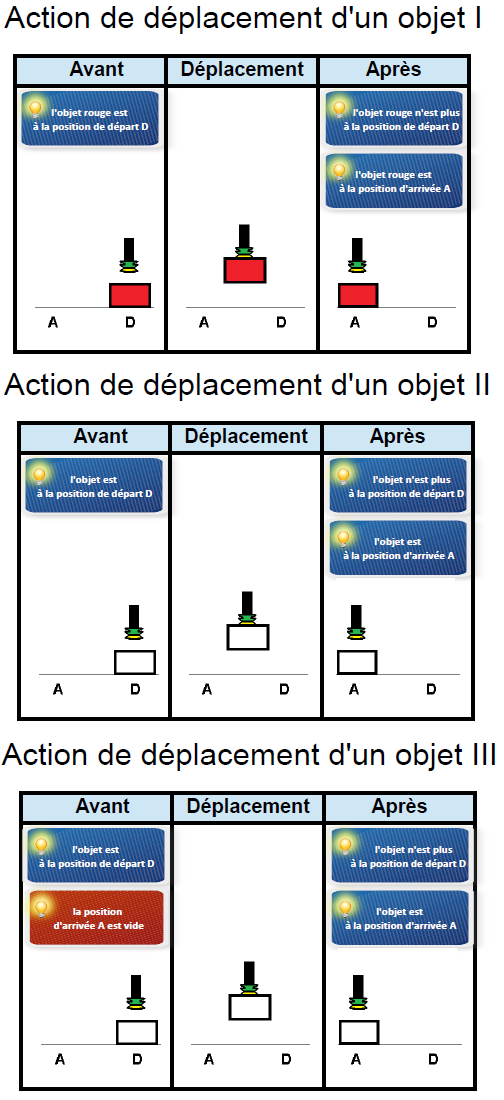
\includegraphics[scale=0.7]{figures/schema-all}
    \caption{Action model used in experiments}
    \label{fig:schema-all}
  \end{figure}


\chapter{Resources for User Evaluation (\chapt{chap:OrganisingTasks})}
\label{app:exp3}
The resources used for evaluating the teaching strategies presented in \chapt{chap:OrganisingTasks} are as follows:
\begin{itemize}
%	\item A demonstration of the Robot Programming process of our proposed framework: \url{https://youtu.be/liaSirH0CeM}
	\item Python code for simulating the teaching strategies: \url{https://github.com/ysl208/organisingtasks/}
	\item The graphical interface used for the AMT user study can be found on Codepen:
	\url{https://codepen.io/ysliang208/project/editor/DYryzp#0}
\end{itemize}
%\section{Experimental protocol}
%
\includepdf[pages=1-7]{7-appendix/exp3-protocole.pdf}
%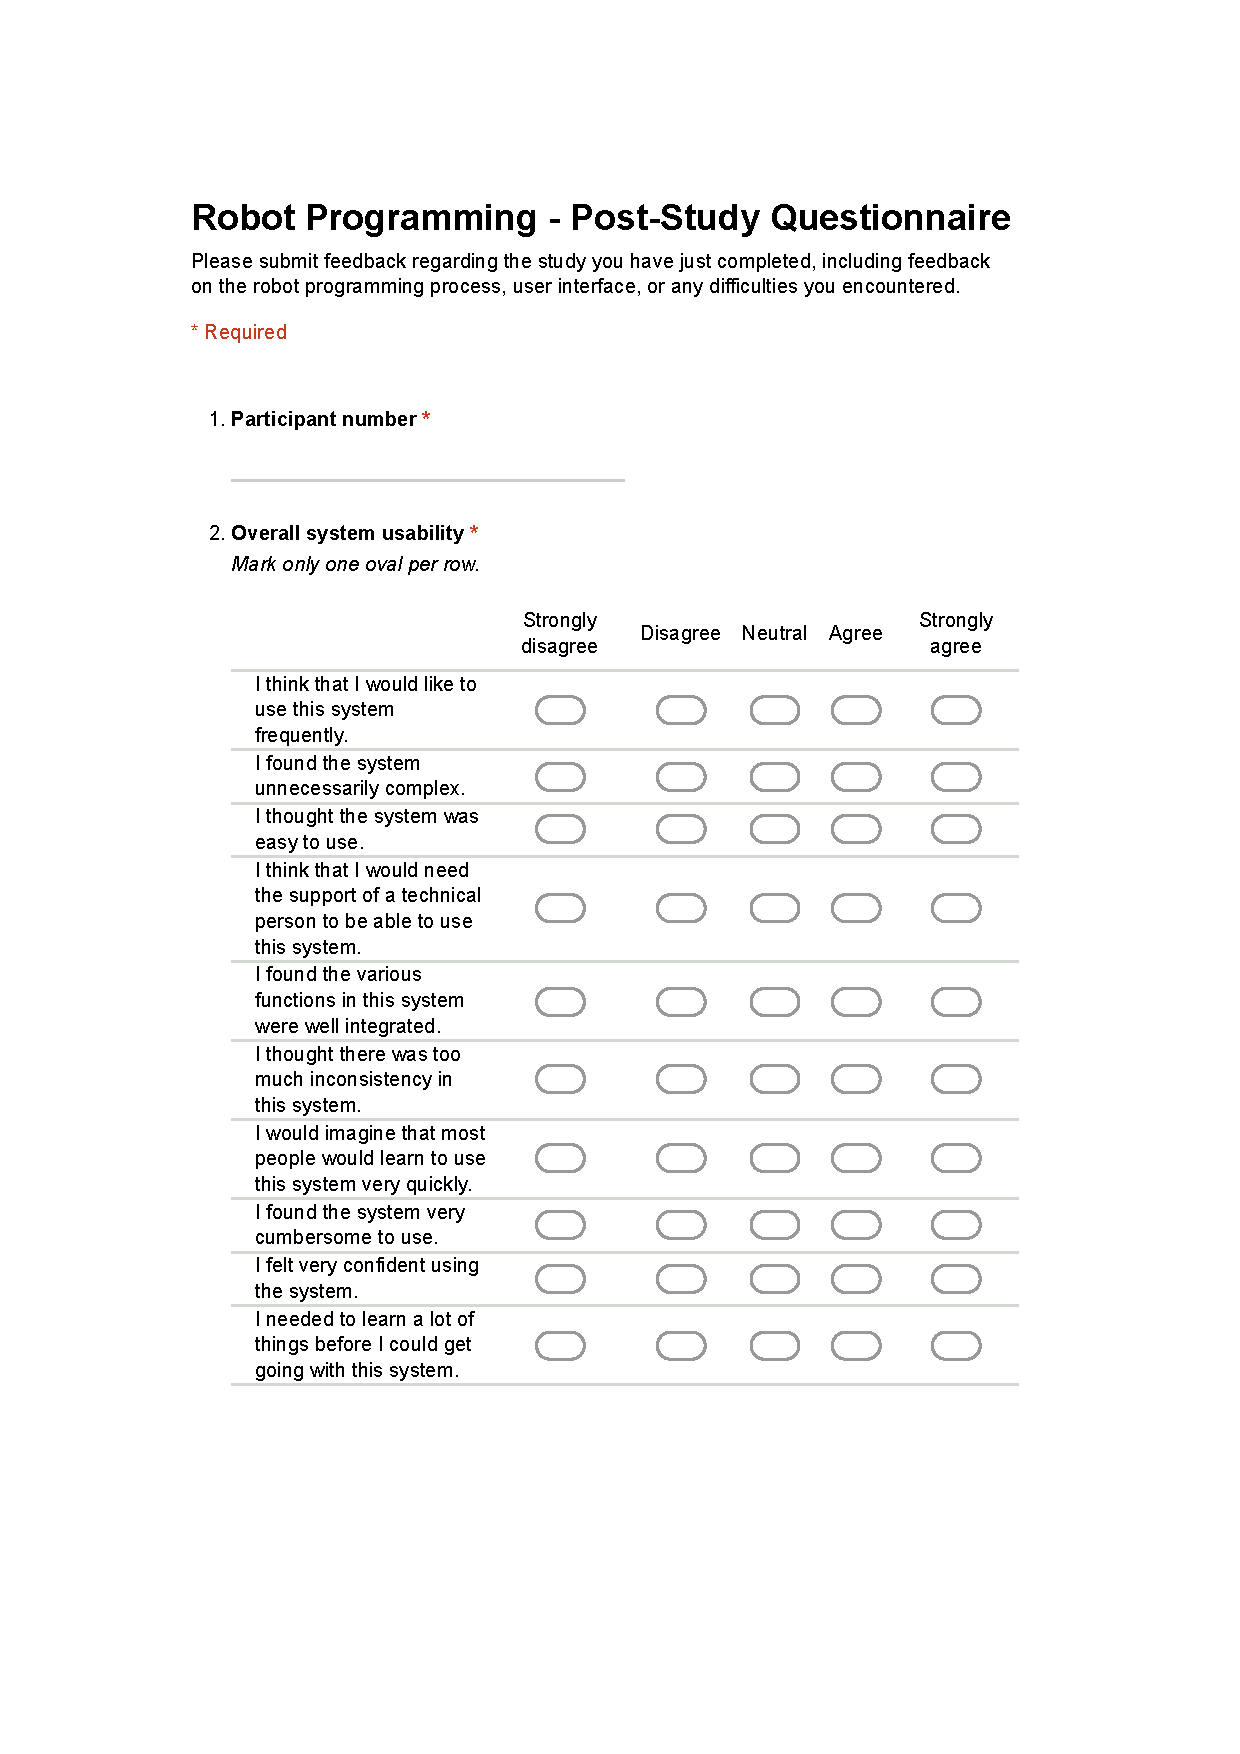
\includepdf[pages=1-3]{7-appendix/exp3-post-questionnaire.pdf}
%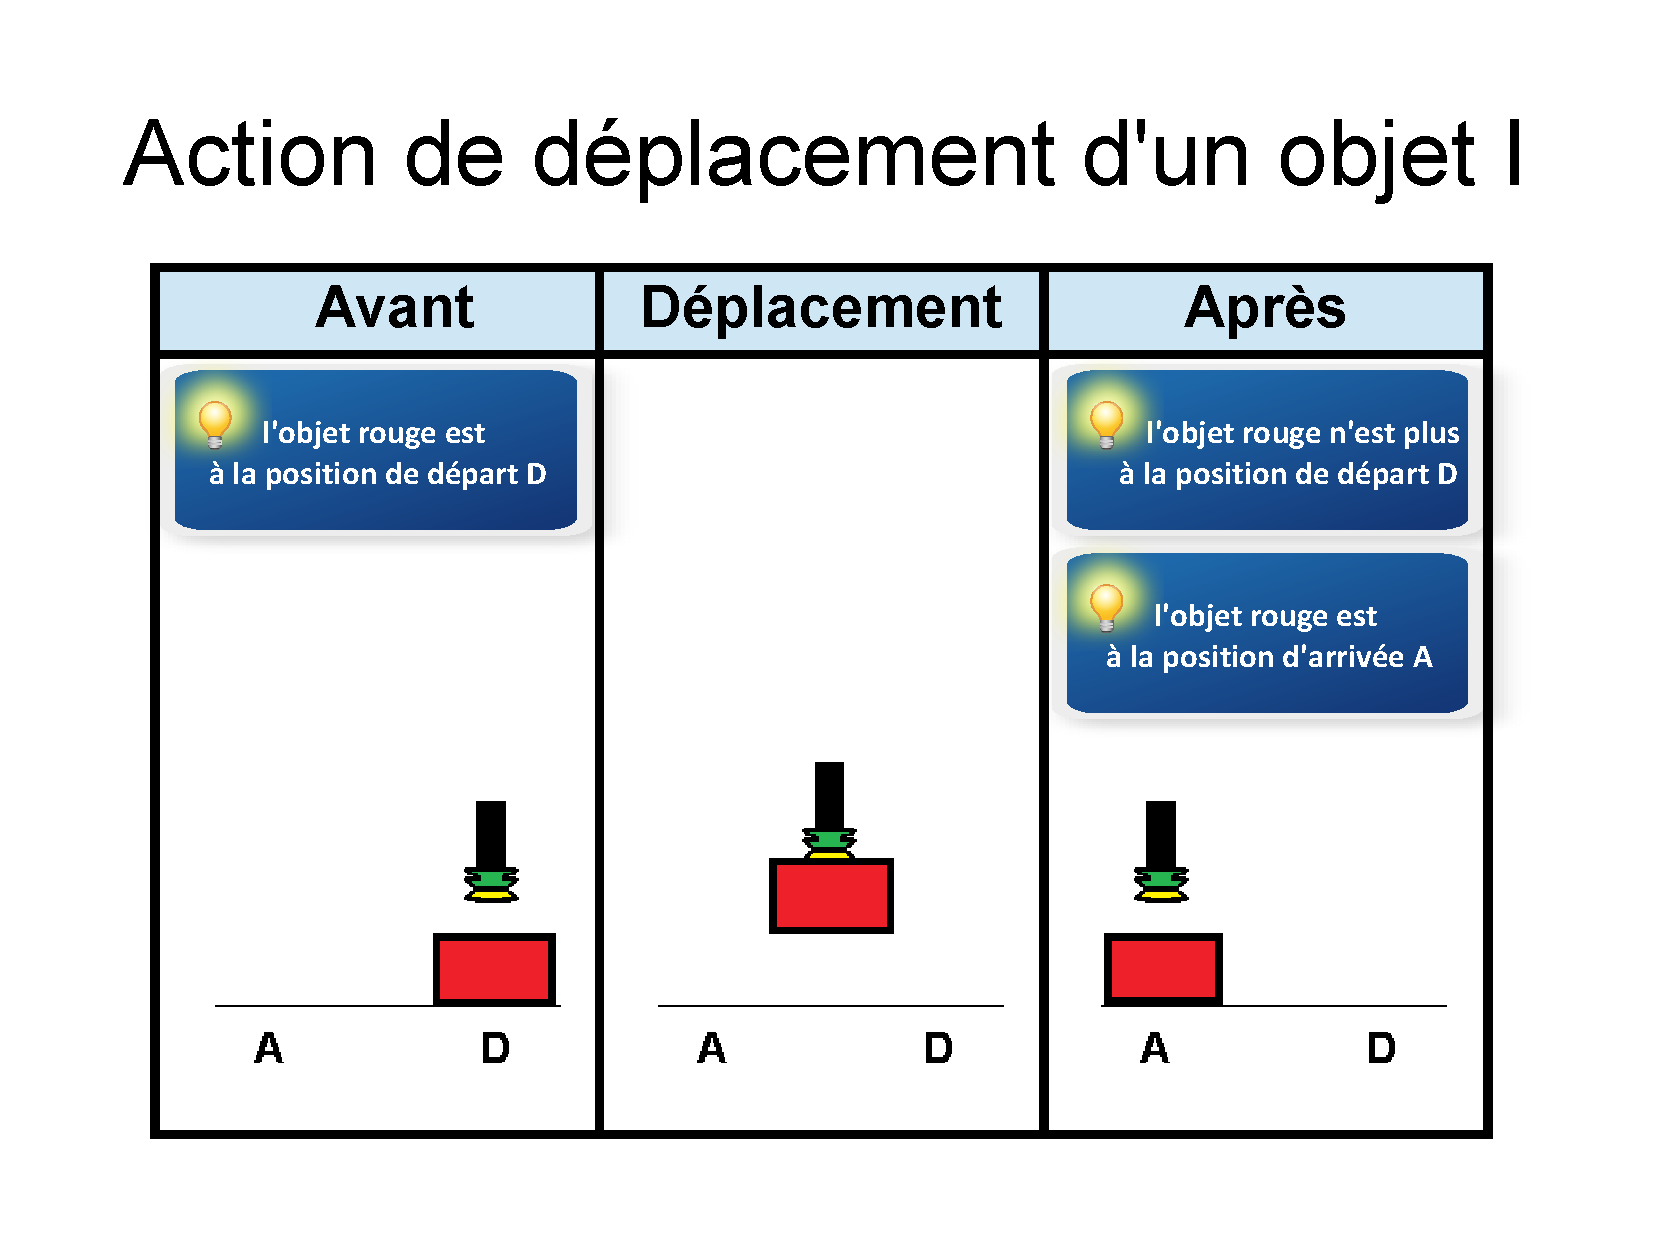
\includepdf[pages=1-3]{7-appendix/exp2-additionalmaterial.pdf}

\chapter{Resources for User Evaluation (\sect{sec:quanteval})}
\label{app:exp4}
The following documents were used in the final user study (all documents are in English):
\begin{itemize}
	\item{THEDRE brainstorming guide}
	\item{THEDRE experimental protocol guide}
	\item{Slides used during the experiment for introduction and tasks}
	\item{Pre-study questionnaire}
	\item{Post-study questionnaire: including questions from the SUS}
%\end{itemize}
%A summary of the resources used for this section can be found online:
%\begin{itemize}
%	\item A demonstration of the Robot Programming process of our proposed framework: \url{https://youtu.be/DTm2YjiSNQM}
	\item The source code for the iRoPro system implementation can be found online: \url{https://github.com/ysl208/iRoPro/tree/cond}
\end{itemize}
%\section{Experimental protocol}
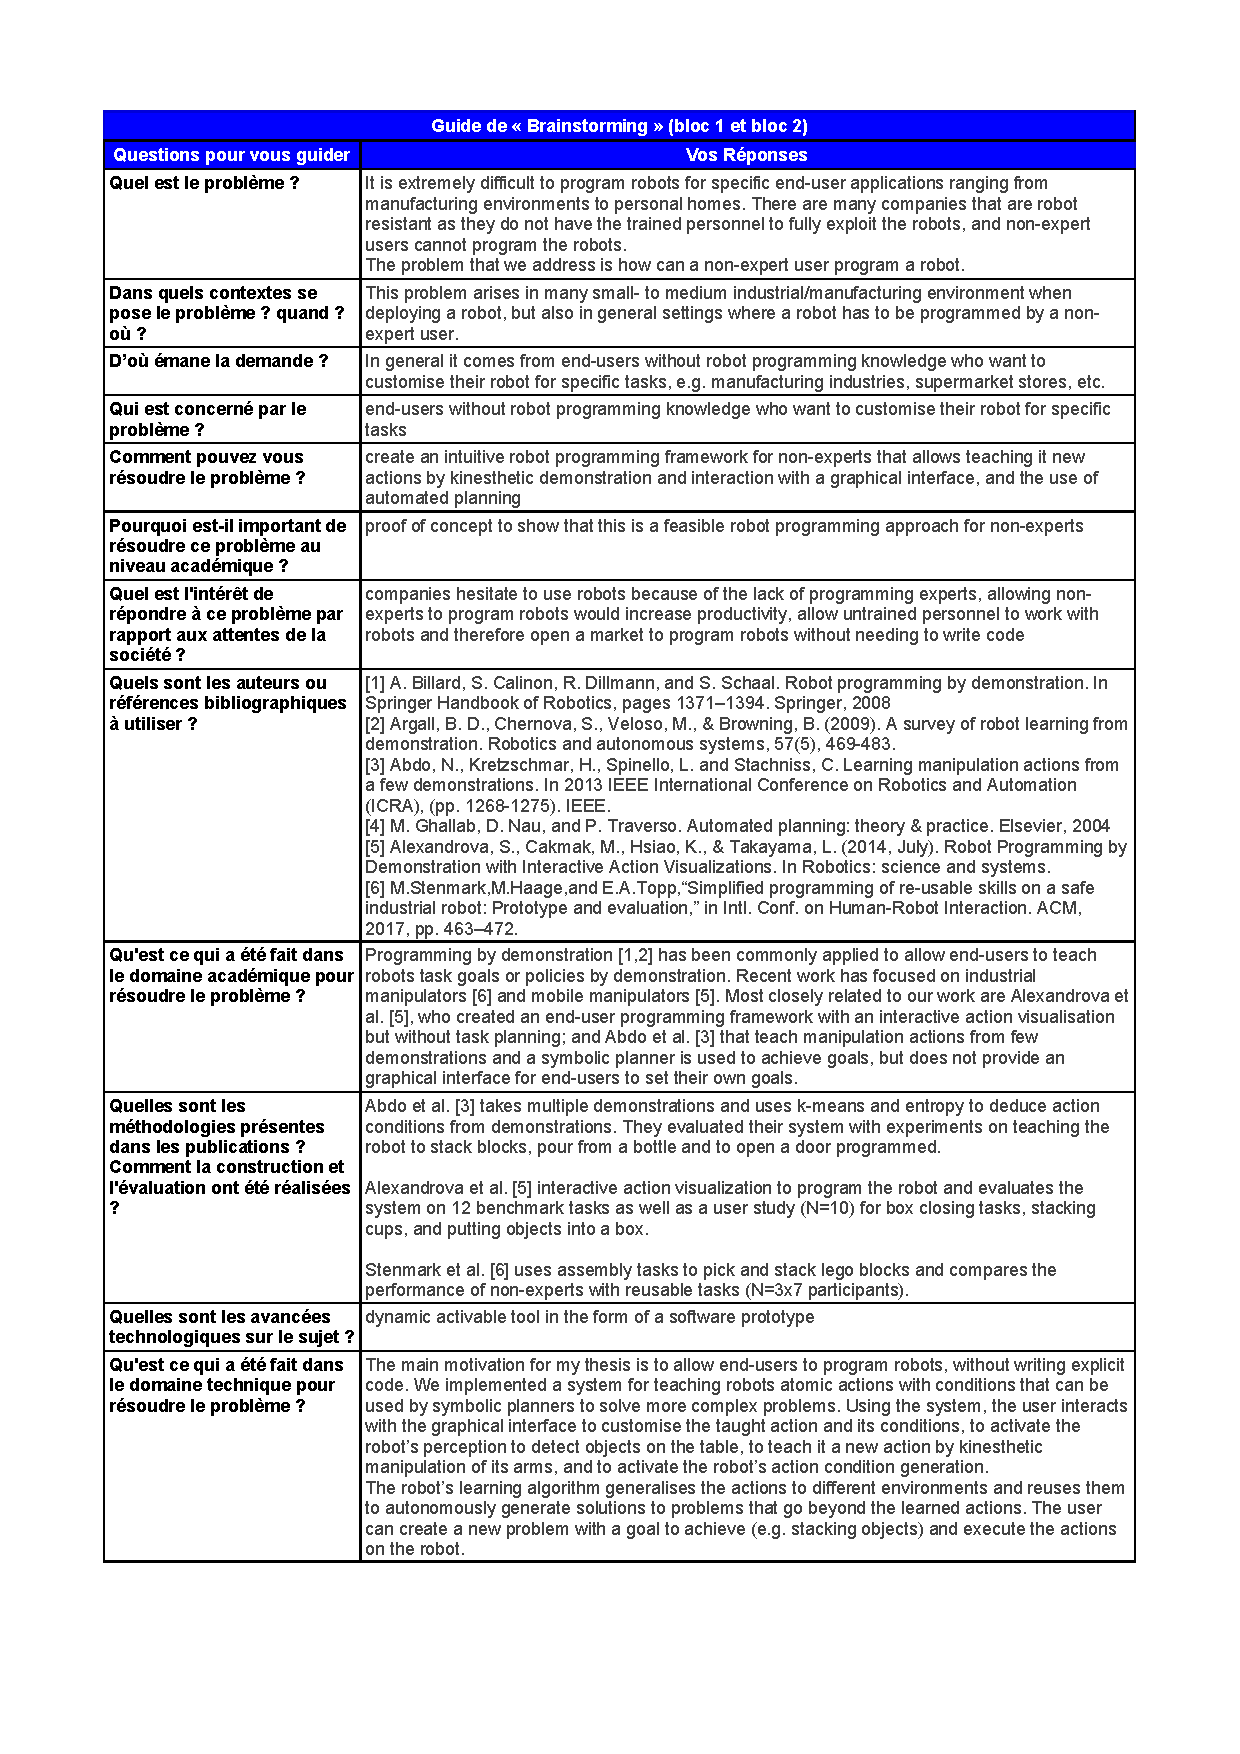
\includepdf[pages=1-2]{7-appendix/exp4-Brainstorming.pdf}
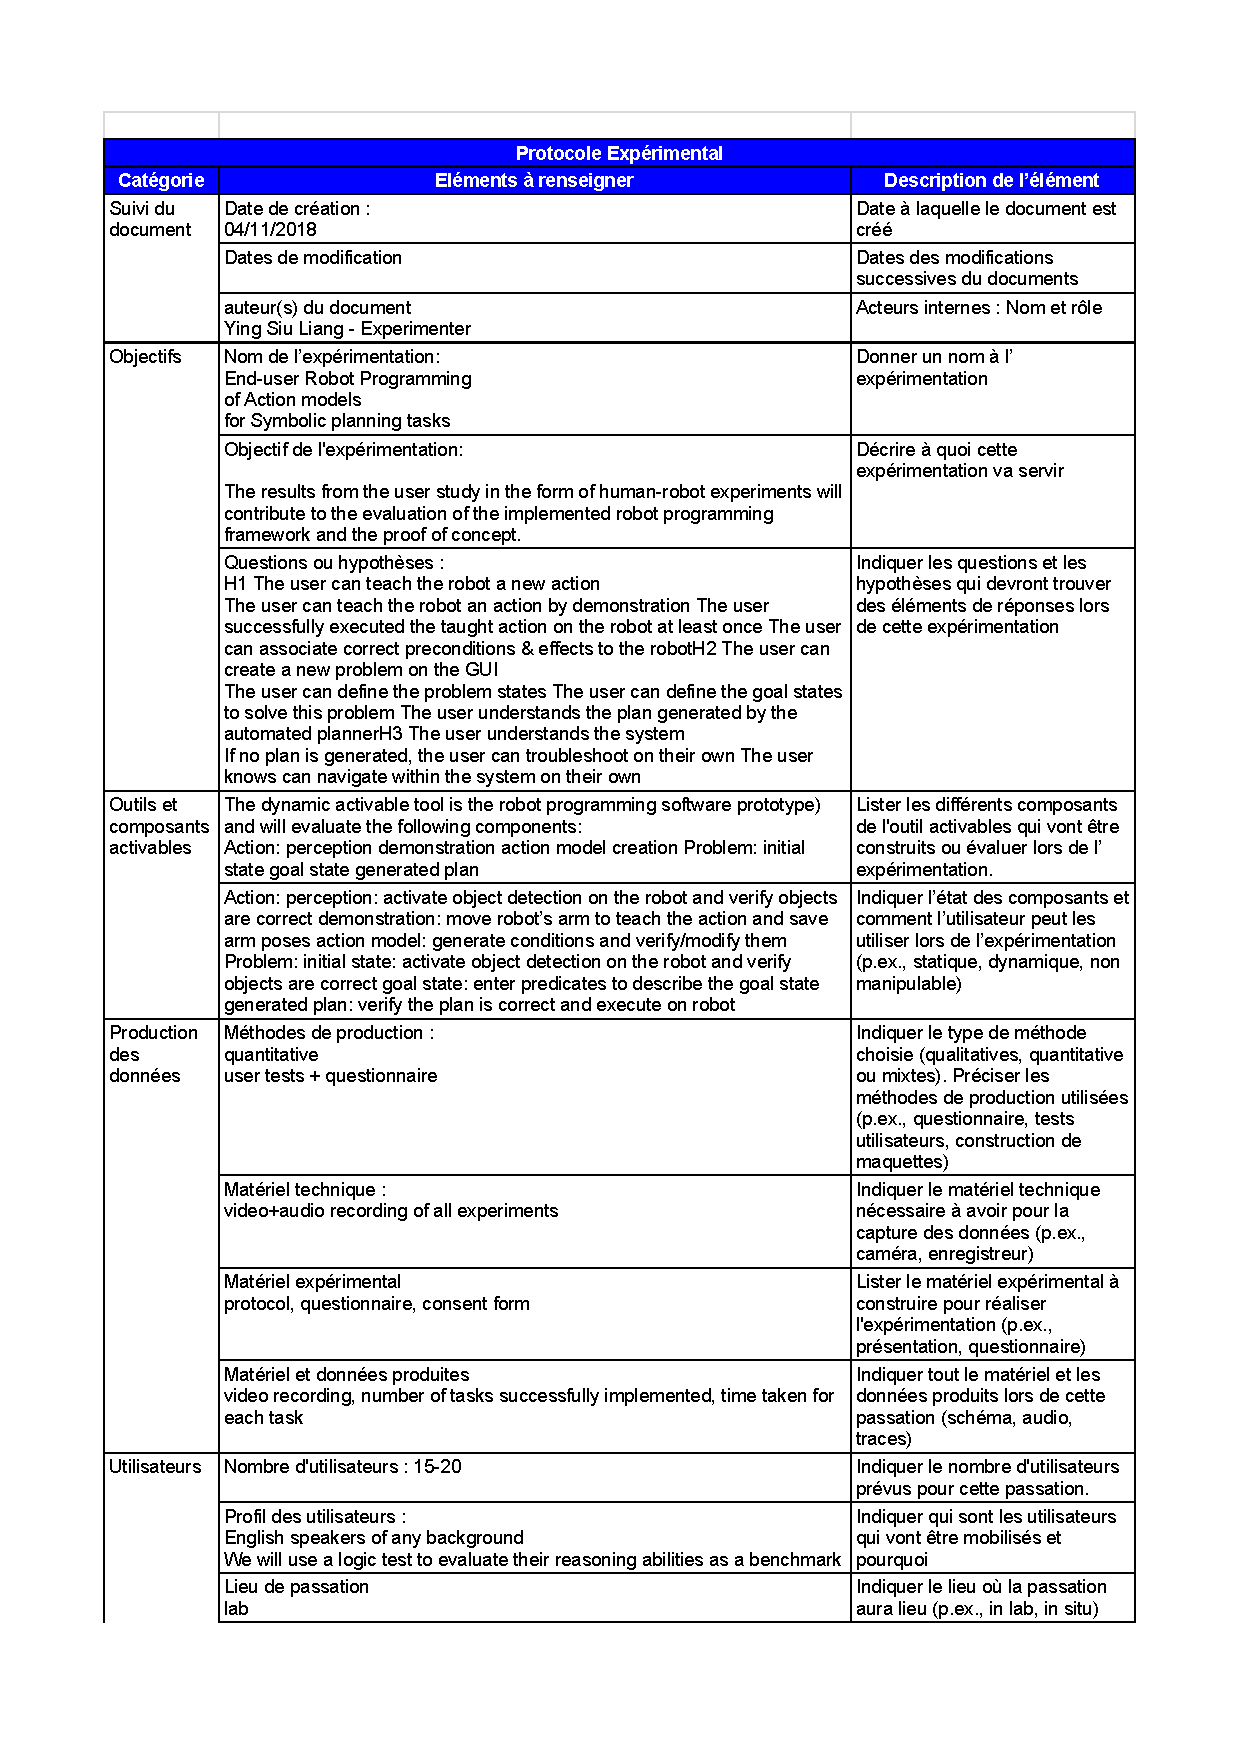
\includepdf[pages=1-2]{7-appendix/exp4-Protocole-Experimental.pdf}
\includepdf[pages=1-7]{7-appendix/exp4-protocole.pdf}
%\section{Questionnaire (In French)}
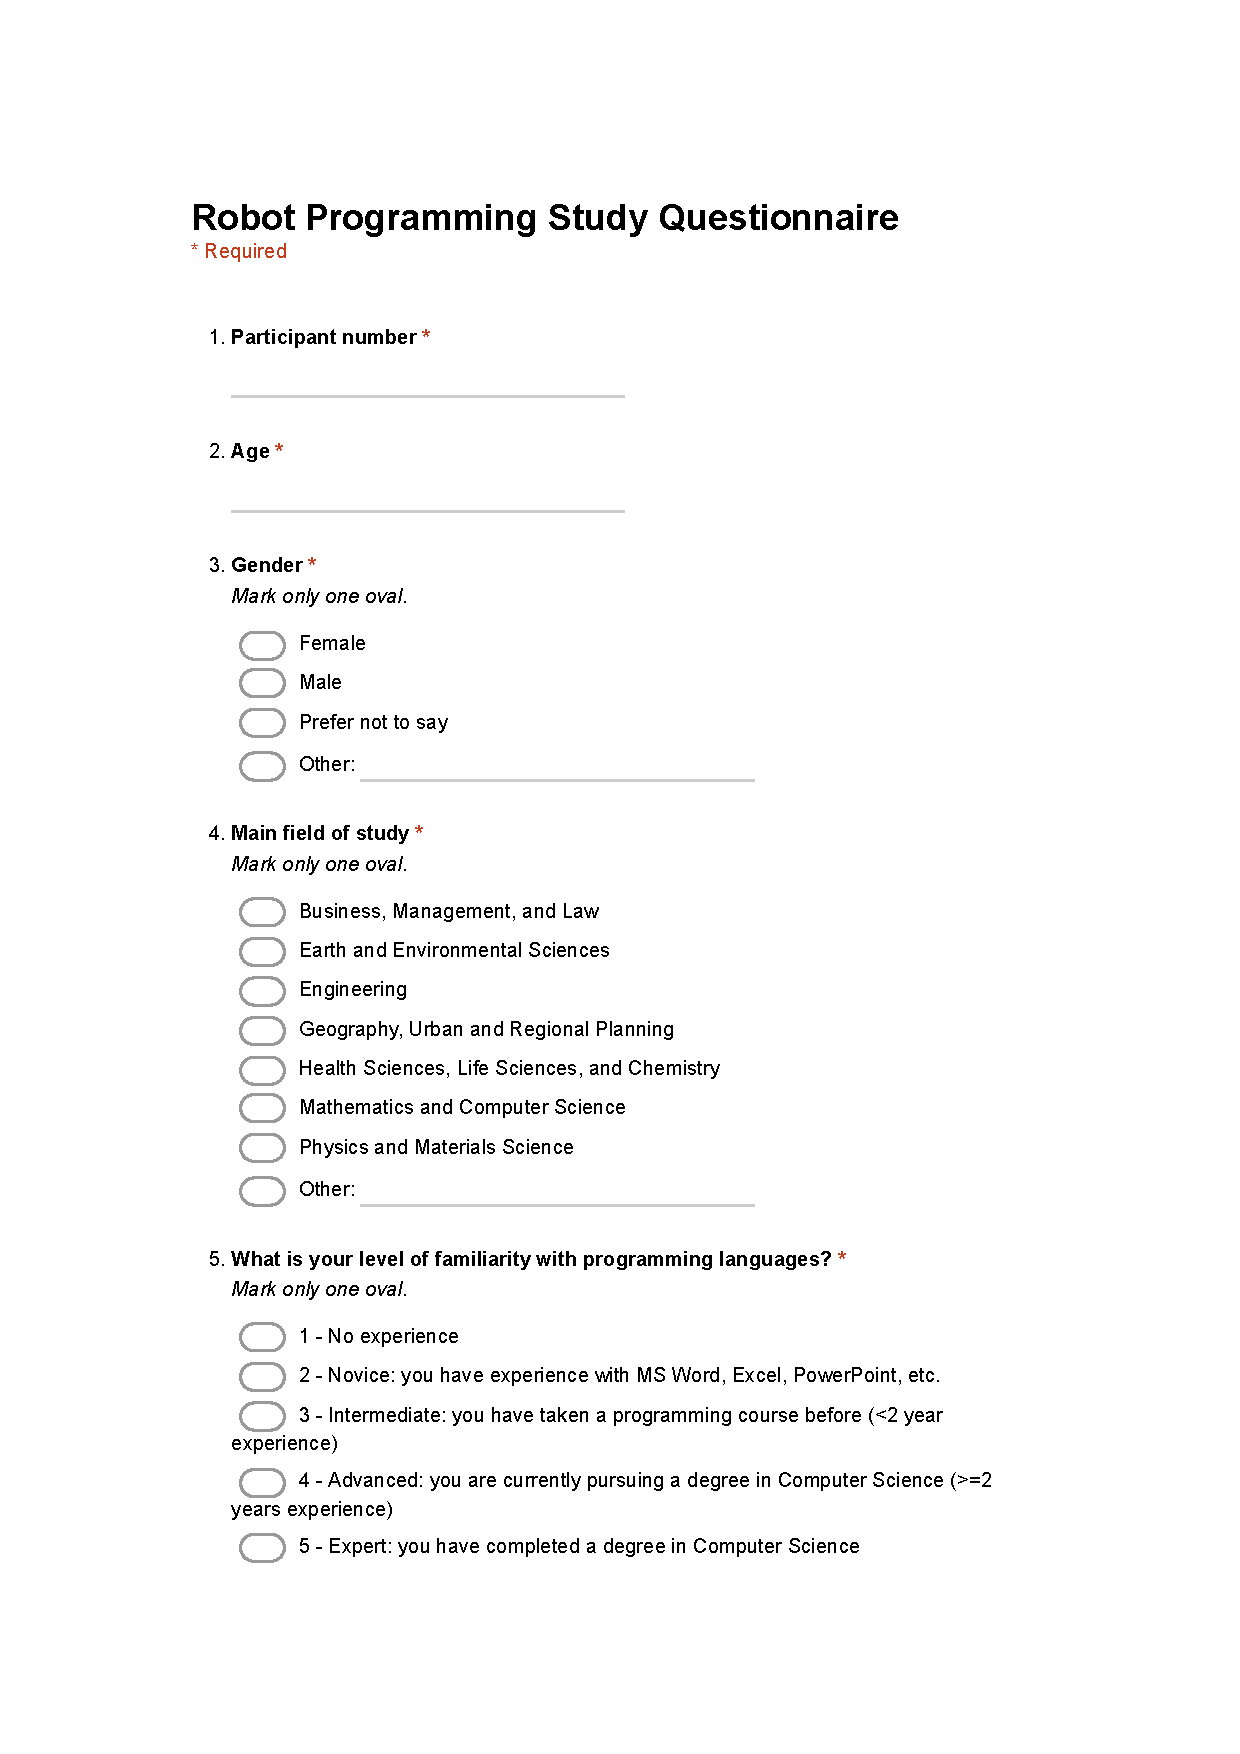
\includepdf[pages=1-3]{7-appendix/exp4-pre-questionnaire.pdf}
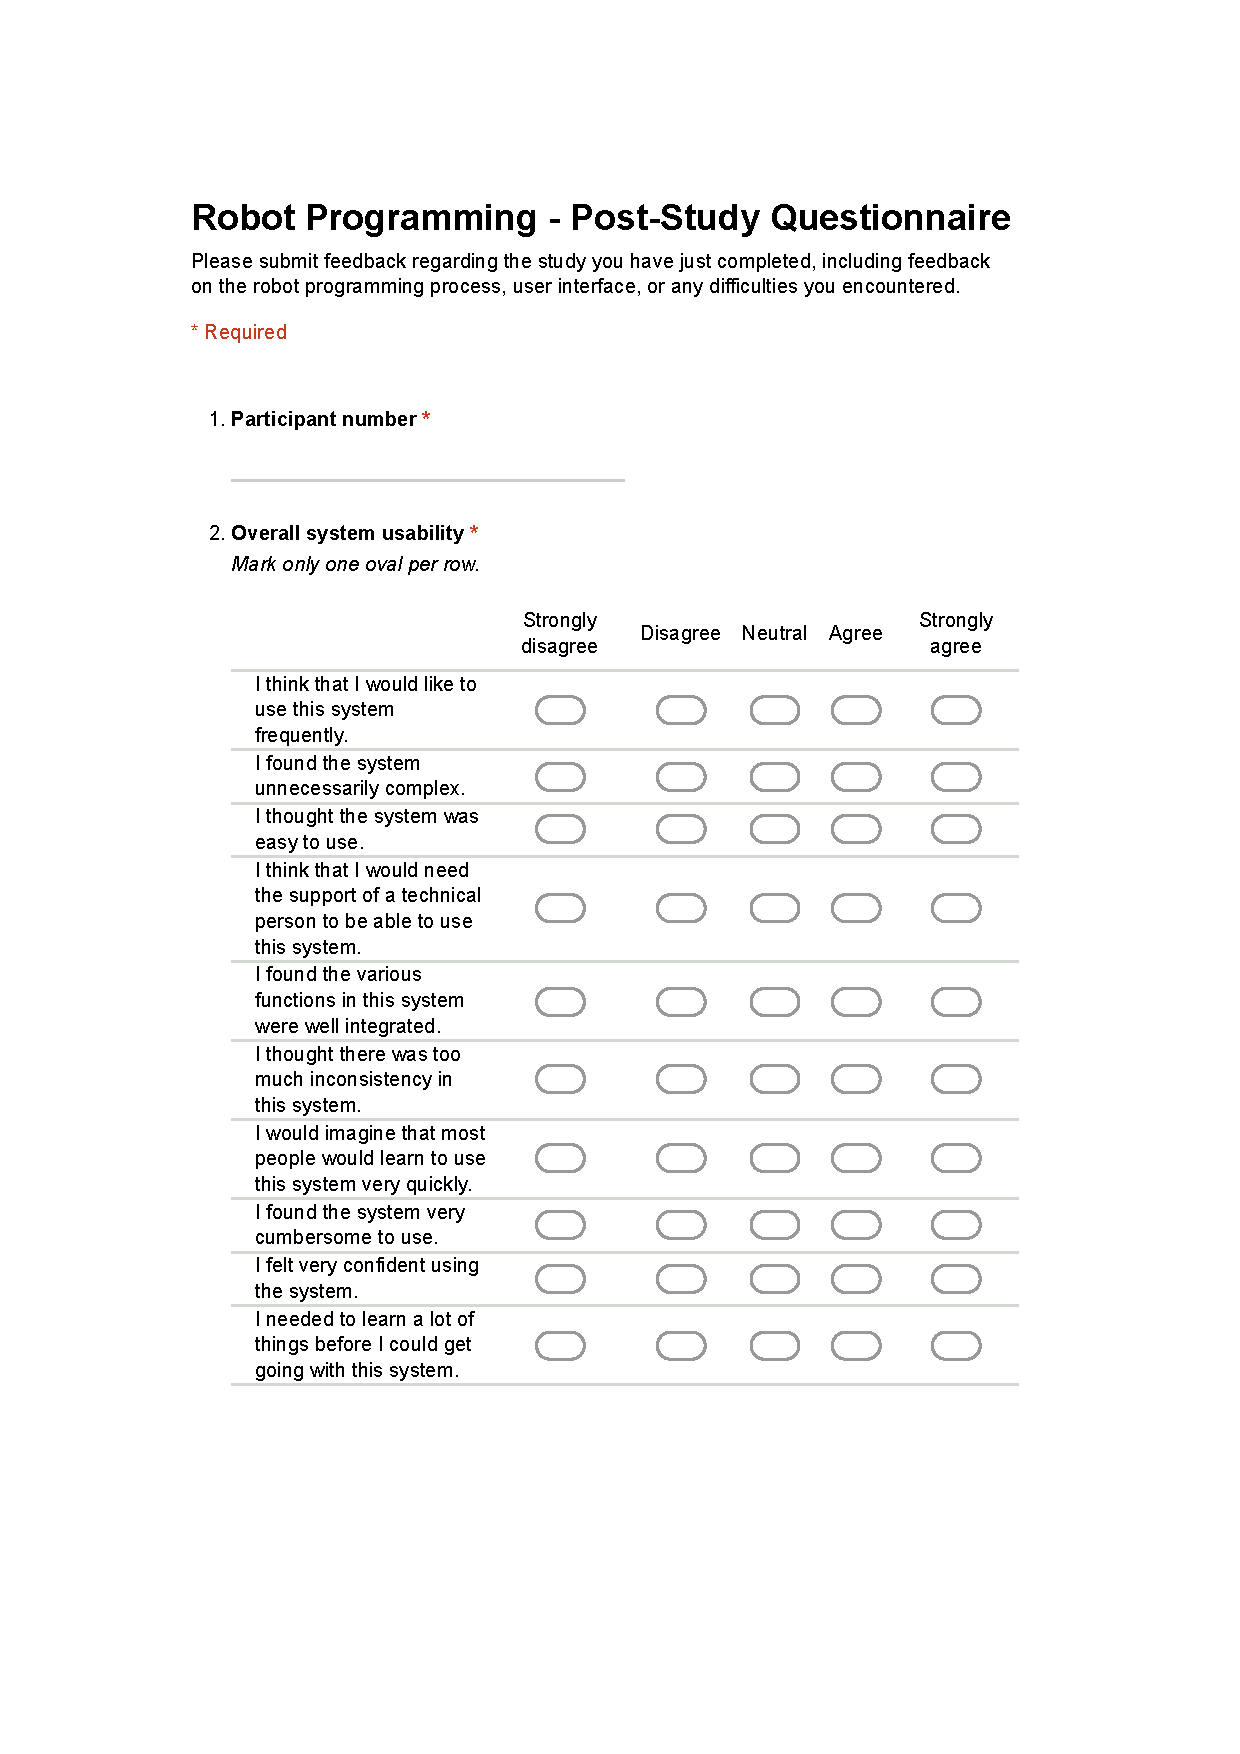
\includepdf[pages=1-3]{7-appendix/exp4-post-questionnaire.pdf}
%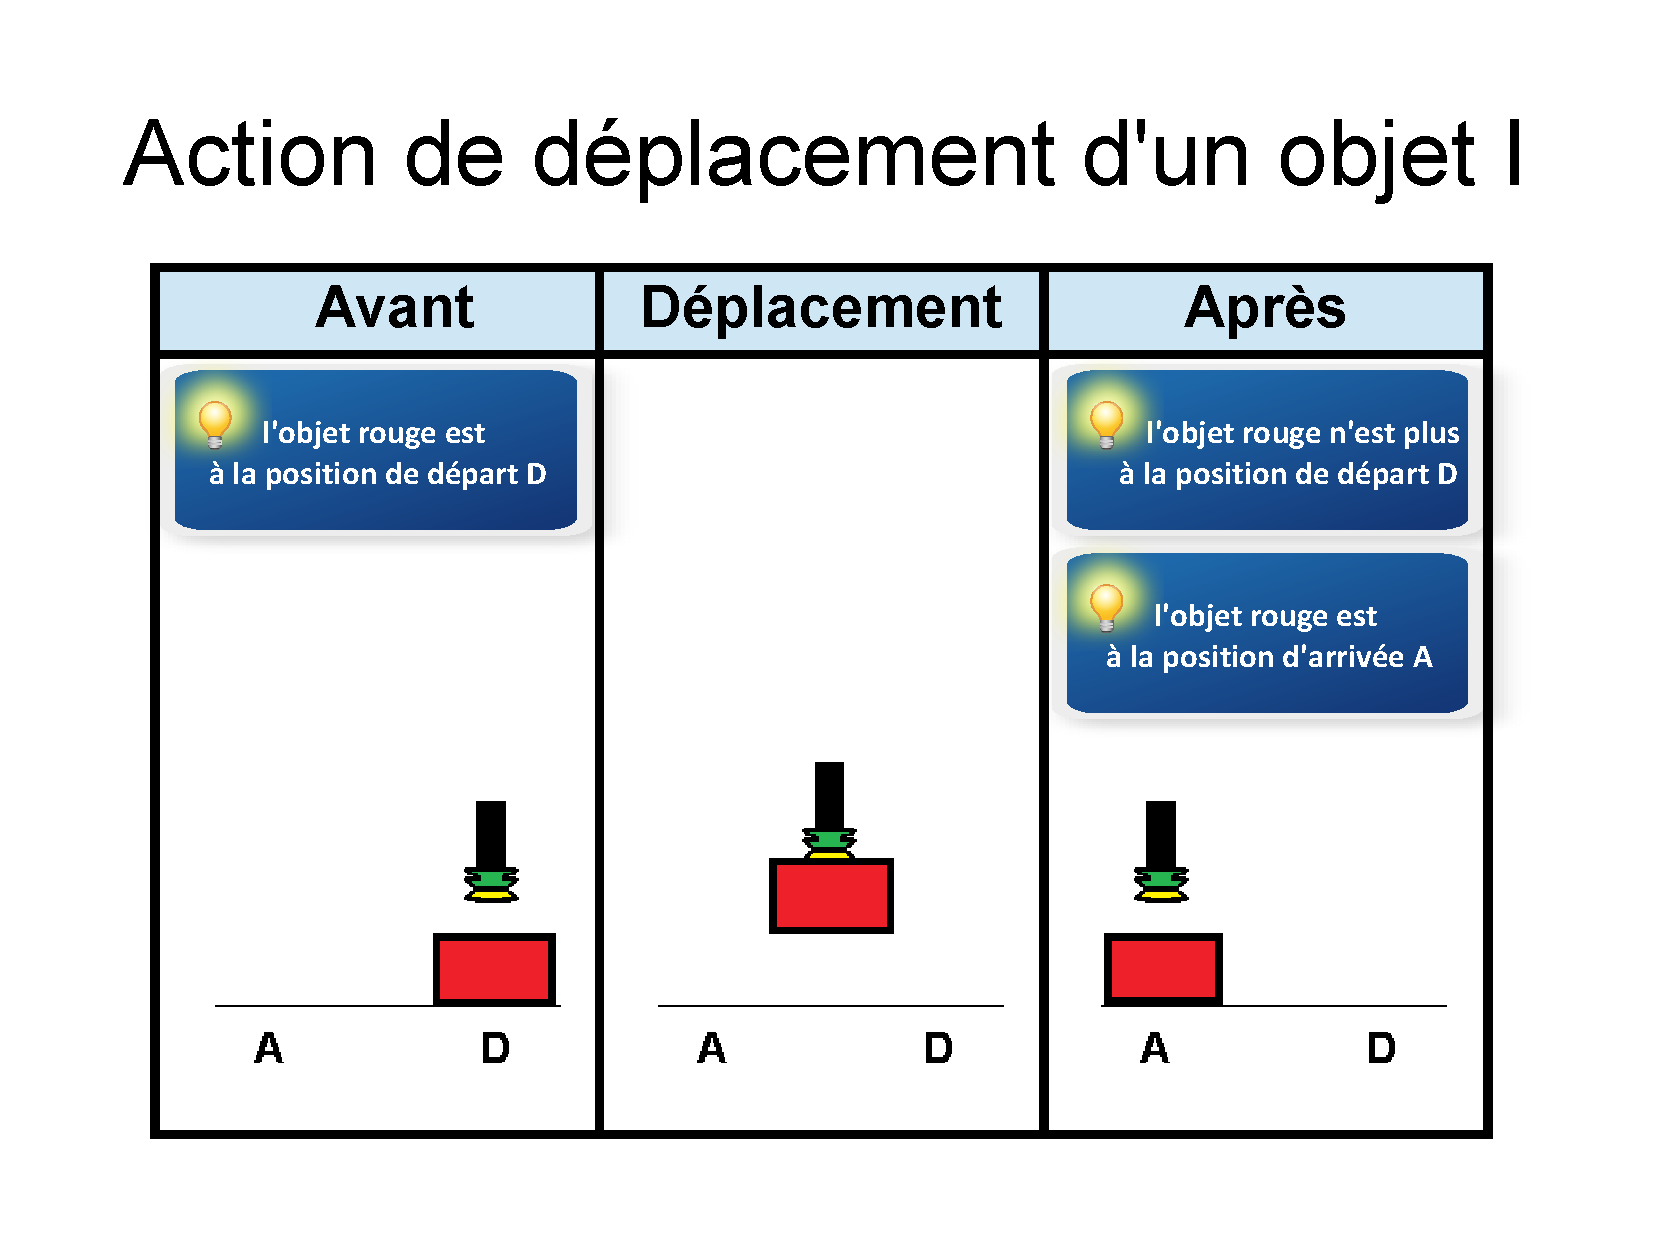
\includepdf[pages=1-3]{7-appendix/exp2-additionalmaterial.pdf}

\chapter{PDDL code used in \chapt{chap:Implementation}}\label{app:pddl}    
\section{iRoPro planning domain}
\begin{verbatim}
(define (domain iRoPro)
(:requirements :typing :strips)
(:types 
  element 
  position - element 
  object - element 
  cube - object 
  base - object 
  roof - object )

(:predicates
  (clear ?e - element)
  (thin ?e - element)
  (flat ?e - element)
  (on ?obj2 - object ?obj1 - element)
  (stackable ?obj2 - object ?obj1 - element) 
)

(:action move-vacuum
  :parameters (?obj - object ?fromLoc - element ?toLoc - element)
  :precondition (and (on ?obj ?fromLoc)
    (clear ?toLoc)
    (not(clear ?fromLoc))
    (flat ?obj)
    (stackable ?obj ?toLoc)
    (clear ?obj) )
  :effect (and (on ?obj ?toLoc)
    (not(clear ?toLoc))
    (clear ?fromLoc)
    (not(on ?obj ?fromLoc)) )
)

(:action move-grip
  :parameters (?obj - object ?fromLoc - element ?toLoc - element)
  :precondition (and (on ?obj ?fromLoc)
    (clear ?toLoc)
    (not(clear ?fromLoc))
    (thin ?obj)
    (stackable ?obj ?toLoc)
    (clear ?obj) )
  :effect (and (on ?obj ?toLoc)
    (not(clear ?toLoc))
    (clear ?fromLoc)
    (not(on ?obj ?fromLoc)) )
)

(:action side-pp
   :parameters (?obj - object ?fromLoc - element ?toLoc - element)
   :precondition (and (on ?obj ?fromLoc)
      (clear ?toLoc)
      (thin ?obj)
      (stackable ?obj ?fromLoc)
      (not(clear ?obj)) )
   :effect (and (on ?obj ?toLoc)
      (not(clear ?fromLoc))
      (clear ?fromLoc)
      (not(on ?obj ?fromLoc)) )
)
)
\end{verbatim}

\section{iRoPro planning problems}
\begin{verbatim}
(define (problem study-task3-swap)
(:domain iRoPro)
(:objects 
  posA posB posC posM - position
  obj1 obj2 - base)
(:init (clear obj1) (on obj1 posA) (clear obj2) (on obj2 posB) 
  (clear posC) (not(clear posB)) (not(clear posA)) (clear posM) 
  (stackable obj1 obj2) (stackable obj1 posA) (stackable obj1 posB) 
  (stackable obj1 posC) (stackable obj1 posM) (flat obj1) 
  (stackable obj2 obj1) (stackable obj2 posA) (stackable obj2 posB) 
  (stackable obj2 posC) (stackable obj2 posM) (flat obj2) 
  (flat posA) (flat posB) (flat posC) (flat posM))
(:goal (on obj1 posB) (on obj2 posA) )
)

(define (problem blocksworld-task2)
(:domain iRoPro)
(:objects 
  posA posB posC posD posE posM - position
  obj1 - base
  obj2 obj3 obj4 - roof)
(:init (clear obj1) (on obj1 posB) (clear obj2) (on obj2 posM) 
  (clear obj3) (on obj3 posC) (clear obj4) (on obj4 posE) 
  (not(clear posC)) (not(clear posM)) (clear posA) (not(clear posB))
  (clear posD) (not(clear posE)) (stackable obj1 posA) 
  (stackable obj1 posB) (stackable obj1 posC) (stackable obj1 posD) 
  (stackable obj1 posE) (stackable obj1 posM) (flat obj1) 
  (stackable obj2 obj1) (stackable obj2 posA) (stackable obj2 posB) 
  (stackable obj2 posC) (stackable obj2 posD) (stackable obj2 posE) 
  (stackable obj2 posM) (thin obj2) (stackable obj3 obj1) 
  (stackable obj3 posA) (stackable obj3 posB) (stackable obj3 posC) 
  (stackable obj3 posD) (stackable obj3 posE) (stackable obj3 posM) 
  (thin obj3) (stackable obj4 obj1) (stackable obj4 posA) 
  (stackable obj4 posB) (stackable obj4 posC) (stackable obj4 posD) 
  (stackable obj4 posE) (stackable obj4 posM) (thin obj4) (flat posA) 
  (flat posB) (flat posC) (flat posD) (flat posE) (flat posM))
(:goal (and (on obj1 posM) (on obj3 obj1) 
                  (on obj4 obj3) (on obj2 obj4) 
)))

(define (problem blocksworld-task34)
(:domain iRoPro)
(:objects 
   posA posB posC posD posE posM - position
   obj1 obj2 obj3 obj4 - roof)
(:init (clear obj4) (clear posC) (clear posB) (clear posE) 
  (on obj1 obj2) (on obj3 obj1) (on obj4 obj3) (on obj2 posM) 
  (stackable obj1 posA) (stackable obj1 posB) (stackable obj1 posC) 
  (stackable obj1 posD) (stackable obj1 posE) (stackable obj1 posM) 
  (thin obj1) (stackable obj2 posA) (stackable obj2 posB) 
  (stackable obj2 posC) (stackable obj2 posD) (stackable obj2 posE) 
  (stackable obj2 posM) (thin obj2) (stackable obj3 posA) 
  (stackable obj3 posB) (stackable obj3 posC) (stackable obj3 posD) 
  (stackable obj3 posE) (stackable obj3 posM) (thin obj3) 
  (stackable obj4 posA) (stackable obj4 posB) (stackable obj4 posC) 
  (stackable obj4 posD) (stackable obj4 posE) (stackable obj4 posM) 
  (thin obj4) (flat posA) (flat posB) (flat posC) (flat posD) 
  (flat posE) (flat posM))
(:goal (and (on obj1 obj2) (on obj3 obj1) 
                  (on obj4 obj3) (on obj2 posB) 
)))

\end{verbatim}
